\section{Level 3: Paschen--Back regime (strong field)}
When $\mu_B B \gg \zeta$ the Zeeman term dominates, $\vb{L}$ and $\vb{S}$ decouple, and $m_l$,
$m_s$ become good quantum numbers:
\begin{equation}
  E \simeq \mu_B B\,(m_l + g_s m_s) + \zeta\, m_l m_s .
\end{equation}
The crossover scale is $B^\ast = \zeta/\mu_B$. Levels with the same $m_j=m_l+m_s$ never cross
(they repel); levels with different $m_j$ may. The two stretched states
$\ket{m_l=\pm1, m_s=\pm\frac12}$ are exact eigenstates at every field,
$E = \zeta/2 \pm \mu_B B (1+g_s/2)$, which the tests use as an exact check.

\begin{figure}[h]
\centering
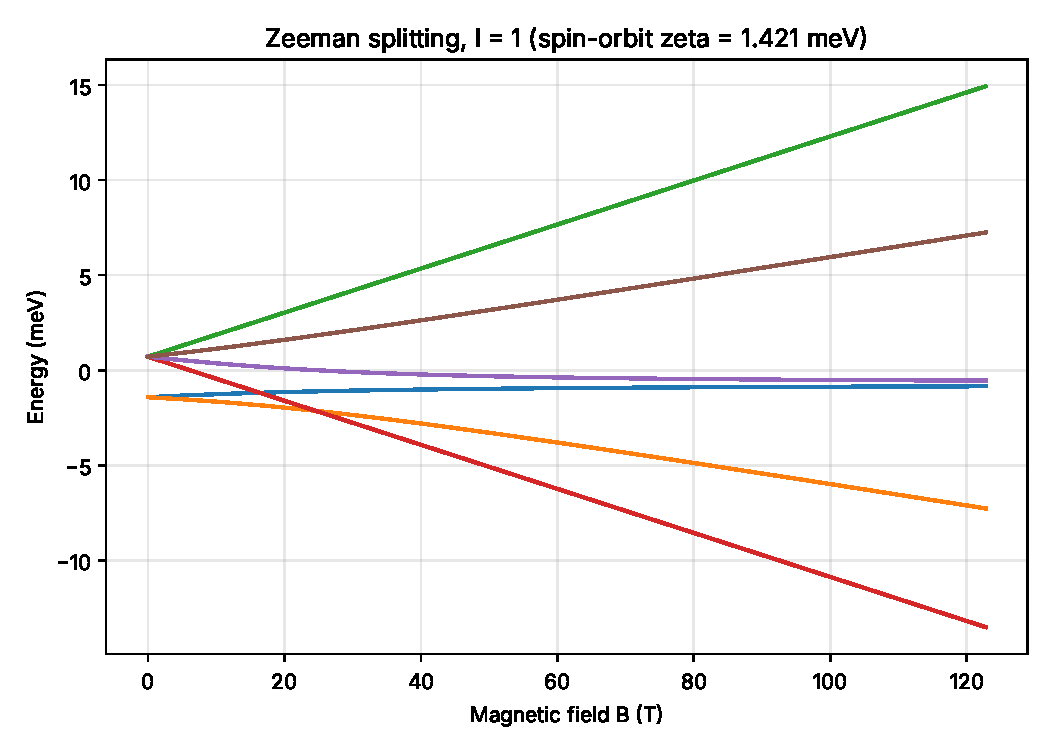
\includegraphics[width=0.8\textwidth]{p_orbital_levels.pdf}
\caption{Energy levels of a $p$ electron (sodium $3p$ spin--orbit constant) from weak field to Paschen--Back.}
\end{figure}
